% Just The Docs Front Matter
% title: Plotting in MATLAB
% parent: Plotting
% nav_order: 1
% has_children: false
% has_toc: false

\subsection{Plotting in MATLAB} \label{sec:getting-started-matlab-plotting} 
\subsubsection{plotmodel}%{{{
\lstinlinebg|plotmodel| takes the model \lstinlinebg|md| as first argument and then an even number of options (as in the function \lstinlinebg|setelementstype|, or \lstinlinebg|solve|). To plot a given field, use the option \lstinlinebg|'data'| followed by the field one wants to plot. For the thickness:
\begin{lstlisting}
>> plotmodel(md, 'data', md.geometry.thickness)
\end{lstlisting}
You can plot several fields at the same time but you have to add the argument \lstinlinebg|'data'| before each field you want to plot:
\begin{lstlisting}
>> plotmodel(md, 'data', md.geometry.thickness, 'data', 'mesh', 'data', [1:md.mesh.numberofelements])
\end{lstlisting}
\begin{figure}[H]
	\begin{center}
		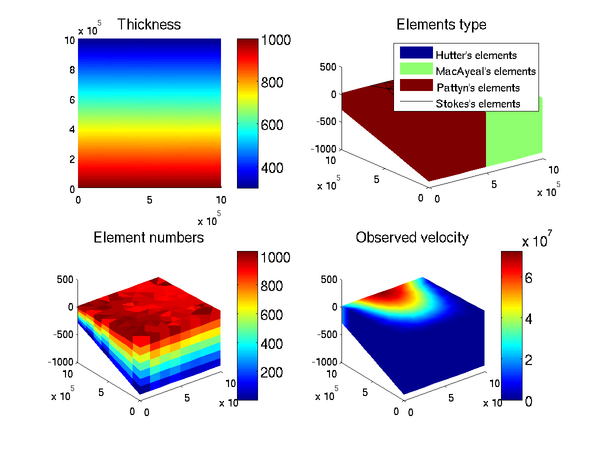
\includegraphics[width=\textwidth]{\assetsParentPath/assets/img/getting-started/plotting/matlab/plot.png}
	\end{center}
\end{figure}
This can work for any field of length \lstinlinebg|md.mesh.numberofelements| or \lstinlinebg|md.mesh.numberofvertices|.
%}}}
\subsubsection{Options}%{{{
Options in \lstinlinebg|plotmodel| come as pairs: the option name must be followed by its value. For example, if one wants to remove the color bar, the option name is \lstinlinebg|'colorbar'| and the value \lstinlinebg|0|:
\begin{lstlisting}
>> plotmodel(md, 'data', md.initialization.vel, 'colorbar', 0)
\end{lstlisting}
any options (except \lstinlinebg|'data'|) can be followed by \lstinlinebg|'#<i>'| where \lstinlinebg|<i>| is the subplot number, or \lstinlinebg|'#all'| if applied to all plots. For example:
\begin{lstlisting}
>> plotmodel(md, 'data', md.initialization.vel, 'data', 'mesh', 'view#2', 3, 'colorbar#all', 'on', 'axis#1', 'off equal')
\end{lstlisting}

\paragraph{axis}
Same as standard \href{http://www.mathworks.com/help/techdoc/ref/axis.html}{axis} MATLAB option:
\begin{lstlisting}
>> plotmodel(md, 'data', md.vel, 'axis', 'tight')
\end{lstlisting}

\paragraph{view}
Same as standard \href{http://www.mathworks.com/help/techdoc/ref/view.html}{view} MATLAB option:
\begin{lstlisting}
>> plotmodel(md, 'data', md.vel, 'view', 2)
\end{lstlisting}

\paragraph{xlim, ylim, zlim}
Same as standard \href{http://www.mathworks.com/help/techdoc/ref/xlim.html}{xlim} MATLAB option:
\begin{lstlisting}
>> plotmodel(md, 'data', md.vel, 'xlim', [10^5 2*10^5])
\end{lstlisting}

\paragraph{caxis}
Same as standard \href{http://www.mathworks.com/access/helpdesk/help/techdoc/index.html?/access/helpdesk/help/techdoc/ref/caxis.html}{caxis} MATLAB option (control the extreme values of the colorbar):
\begin{lstlisting}
>> plotmodel(md, 'data', md.vel, 'caxis', [0 1000])
\end{lstlisting}
\begin{figure}[H]
	\begin{center}
		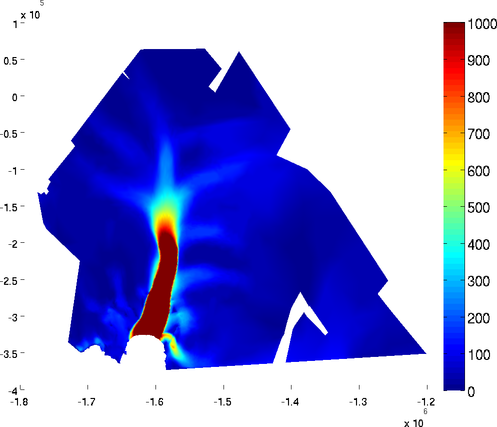
\includegraphics[width=\textwidth]{\assetsParentPath/assets/img/getting-started/plotting/matlab/caxis.png}
	\end{center}
\end{figure}

\paragraph{colorbar}
This option is used to control the colorbar display (\lstinlinebg|'on'| or \lstinlinebg|'off'|):
\begin{lstlisting}
>> plotmodel(md, 'data', md.vel, 'colorbar', 'off')
\end{lstlisting}

\paragraph{colormap}
Same as standard \href{http://www.mathworks.com/access/helpdesk/help/techdoc/index.html?/access/helpdesk/help/techdoc/ref/colormap.html}{colormap} MATLAB option (control the extreme values of the colorbar):
\begin{lstlisting}
>> plotmodel(md, 'data', md.vel, 'colormap', 'hsv')
\end{lstlisting}
\begin{figure}[H]
	\begin{center}
		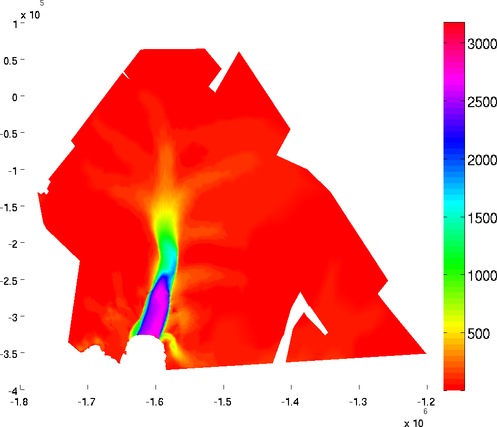
\includegraphics[width=\textwidth]{\assetsParentPath/assets/img/getting-started/plotting/matlab/colormap.png}
	\end{center}
\end{figure}

\paragraph{log}
To get a logarithmic colorbar, use the \lstinlinebg|'log'| option followed by \lstinlinebg|10| for a decimal logarithm:
\begin{lstlisting}
>> plotmodel(md, 'data', md.vel, 'log', 10)
\end{lstlisting}
\begin{figure}[H]
	\begin{center}
		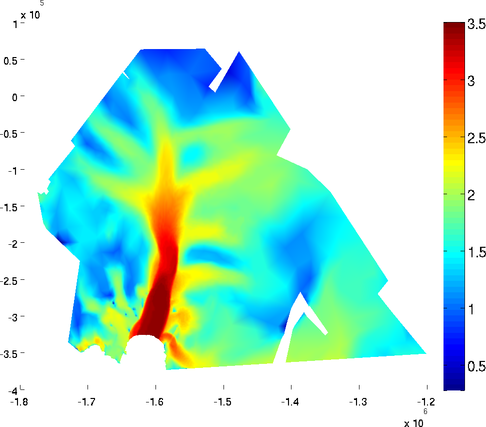
\includegraphics[width=\textwidth]{\assetsParentPath/assets/img/getting-started/plotting/matlab/log.png}
	\end{center}
\end{figure}

\paragraph{contourlevels}
Contours of equi-value can be added to the plot by using the \lstinlinebg|'contourlevels'| option. The number of contours can be chosen by using the \lstinlinebg|'contourlevels'| options. The user can specify a number of levels or a cell containing the values of color changes. For example:
\begin{lstlisting}
>> plotmodel(md, 'data', md.vel, 'contourlevels', 3)
\end{lstlisting}
\begin{figure}[H]
	\begin{center}
		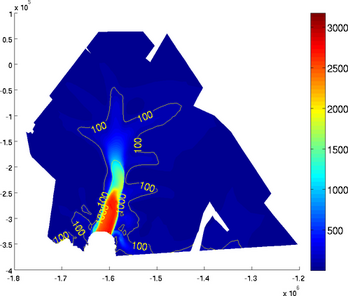
\includegraphics[width=\textwidth]{\assetsParentPath/assets/img/getting-started/plotting/matlab/contour3.png}
	\end{center}
\end{figure}
\begin{lstlisting}
>> plotmodel(md, 'data', md.vel, 'contourlevels', {100, 200, 500, 1000, 2000, 2500})
\end{lstlisting}
\begin{figure}[H]
	\begin{center}
		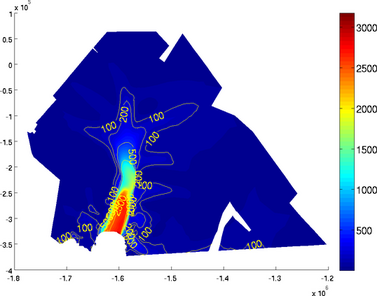
\includegraphics[width=\textwidth]{\assetsParentPath/assets/img/getting-started/plotting/matlab/contourcell.png}
	\end{center}
\end{figure}

\paragraph{contourticks}
If the user does not want to display the contour levels ticks, use the \lstinlinebg|'contourticks'| set as \lstinlinebg|'off'|:
\begin{lstlisting}
>> plotmodel(md, 'data', md.vel, 'contourlevels', {100, 200, 500, 1000, 2000, 2500}, 'contourticks', 'off')
\end{lstlisting}
\begin{figure}[H]
	\begin{center}
		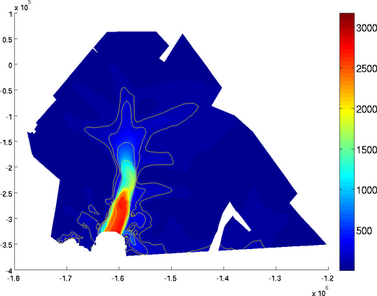
\includegraphics[width=\textwidth]{\assetsParentPath/assets/img/getting-started/plotting/matlab/contourticks.png}
	\end{center}
\end{figure}

\paragraph{contouronly}
If the user wants to display the contours only, use the \lstinlinebg|'contouronly'| set as \lstinlinebg|'on'|:
\begin{lstlisting}
>> plotmodel(md, 'data', 'vel', 'contourlevels', {100, 200, 500, 1000, 2000, 2500}, 'contouronly', 'on')
\end{lstlisting}

\paragraph{streamlines}
Streamlines can be displayed by using the \lstinlinebg|'streamlines'| option followed by a number of streamlines or a cell containing the coordinates of seed points:
\begin{lstlisting}
>> plotmodel(md, 'data', md.initialization.vel, 'streamlines', 50)
\end{lstlisting}
\begin{lstlisting}
>> plotmodel(md, 'data', md.initialization.vel, 'streamlines', {10^6 * [-1.45 -0.27], 10^6 * [-1.6 0]})
\end{lstlisting}
\begin{figure}[H]
	\begin{center}
		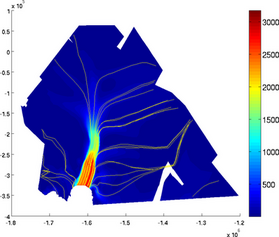
\includegraphics[width=0.475\textwidth]{\assetsParentPath/assets/img/getting-started/plotting/matlab/streamlines50.png}
		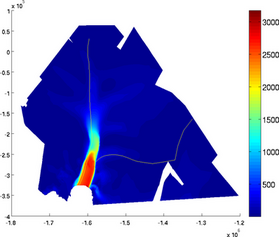
\includegraphics[width=0.475\textwidth]{\assetsParentPath/assets/img/getting-started/plotting/matlab/streamlinescell.png}
	\end{center}
\end{figure}

NOTE: Streamlines use the velocities that are in \lstinlinebg|md.initialization|. Make sure you transfer the calculated velocities to \lstinlinebg|md.initialization| if you want to display the calculated streamlines.

\paragraph{edgecolor}
The mesh can be superimposed onto the plot by using the \lstinlinebg|'edgecolor'| option followed by a color:
\begin{lstlisting}
>> plotmodel(md, 'data', md.initialization.vel, 'edgecolor', 'w')
\end{lstlisting}
\begin{figure}[H]
	\begin{center}
		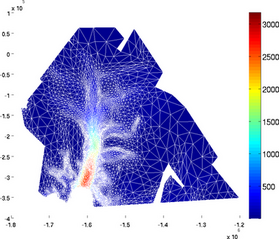
\includegraphics[width=\textwidth]{\assetsParentPath/assets/img/getting-started/plotting/matlab/edgecolor.png}
	\end{center}
\end{figure}

\paragraph{expdisp}
Any ARGUS file can be displayed with the \lstinlinebg|'expdisp'| option followed by the name of the ARGUS file:
\begin{lstlisting}
>> plotmodel(md, 'data', md.initialization.vel, 'expdisp', 'Iceshelves.exp')
\end{lstlisting}

\paragraph{expstyle}
The style of the ARGUS profile can be controlled with the \lstinlinebg|'expstyle'| option, followed by the desired line style. Here is an example for a yellow dotted line:
\begin{lstlisting}
>> plotmodel(md, 'data', md.initialization.vel, 'expdisp', 'Iceshelves.exp', 'expstyle', '--y')
\end{lstlisting}

\paragraph{mask}
If one does not want to display the value of the field on a mask only, use the \lstinlinebg|'mask'| option followed by a vector that holds 0 for the vertices whose values are hidden:
\begin{lstlisting}
>> plotmodel(md, 'data', md.initialization.vel, 'mask', md.mask.ocean_levelset < 0)
\end{lstlisting}
\begin{figure}[H]
	\begin{center}
		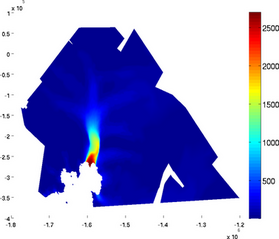
\includegraphics[width=\textwidth]{\assetsParentPath/assets/img/getting-started/plotting/matlab/mask.png}
	\end{center}
\end{figure}

\paragraph{northarrow}
An arrow pointing North can be added with the \lstinlinebg|'northarrow'| option followed by \lstinlinebg|'on'|. The shape and position of the arrow can be controlled by using \lstinlinebg|[x0 y0 length [ratio [width]]]| 
instead of \lstinlinebg|'on'|:
\begin{lstlisting}
>> plotmodel(md, 'data', md.initialization.vel, 'northarrow', 'on')
\end{lstlisting}

\paragraph{scaleruler}
A scale ruler can be added. As for the North arrow, the default display is done by \lstinlinebg|'on'| but the shape and position of the scale ruler can be controlled by \lstinlinebg|[x0 y0 length width numberofticks]| where (x0,y0) are the coordinates of the lower left corner:
\begin{lstlisting}
>> plotmodel(md, 'data', md.initialization.vel, 'scaleruler', 'on')
\end{lstlisting}

\paragraph{title}
Same as standard \href{http://www.mathworks.com/help/techdoc/ref/title.html}{title} MATLAB option:
\begin{lstlisting}
>> plotmodel(md, 'data', md.vel, 'title', 'Ice velocity [m/yr]')
\end{lstlisting}

\paragraph{fontsize}
Same as standard \href{http://www.mathworks.com/help/techdoc/ref/text_props.html}{fontsize} MATLAB option:
\begin{lstlisting}
>> plotmodel(md, 'data', md.vel, 'title', 'Ice velocity [m/yr]', 'fontsize', 8)
\end{lstlisting}

\paragraph{fontweight}
Same as standard \href{http://www.mathworks.com/help/techdoc/ref/text_props.html}{fontweight} MATLAB option:
\begin{lstlisting}
>> plotmodel(md, 'data', md.vel, 'title', 'Ice velocity [m/yr]', 'fontweight', 'b')
\end{lstlisting}

\paragraph{xlabel, ylabel}
Same as standard \href{http://www.mathworks.com/help/techdoc/ref/xlabel.html}{xlabel} MATLAB option:
\begin{lstlisting}
>> plotmodel(md, 'data', md.vel, 'xlabel', 'x axis [m]')
\end{lstlisting}
%}}}
\subsubsection{Special plots}%{{{
\paragraph{basaldrag}%{{{
The special plot \lstinlinebg|'basal_drag'| displays the norm of the basal drag friction in kPa following formula:
\begin{equation}
	\boldsymbol{\tau}_b = -k^2 N^r \|{\bf v}\|^{s-1} {\bf v}_b
\end{equation}
Basal drag relies on the velocity provided in \lstinlinebg|md.initialization|. The x and y components of the basal drag can be displayed with the \lstinlinebg|'basal_dragx'| or \lstinlinebg|'basal_dragy'| special plots:
\begin{lstlisting}
>> plotmodel(md, 'data', 'basal_drag')
\end{lstlisting}
\begin{lstlisting}
>> plotmodel(md, 'data', 'basal_dragx')
\end{lstlisting}
\begin{figure}[H]
	\begin{center}
		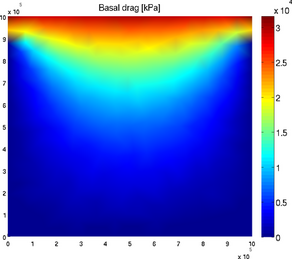
\includegraphics[width=0.475\textwidth]{\assetsParentPath/assets/img/getting-started/plotting/matlab/basaldrag.png}
		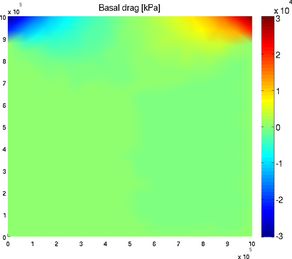
\includegraphics[width=0.475\textwidth]{\assetsParentPath/assets/img/getting-started/plotting/matlab/basaldragcomp.png}
		\caption{Basal friction norm and Basal friction x-component}
	\end{center}
\end{figure}
%}}}

\paragraph{BC}%{{{
The special plot \lstinlinebg|'BC'| displays all boundary conditions (Newmann and Dirichlet) for 2D and 3D meshes:
\begin{lstlisting}
>> plotmodel(md, 'data', 'BC')
\end{lstlisting}
\begin{figure}[H]
	\begin{center}
		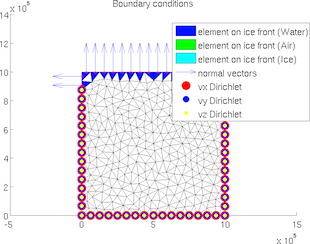
\includegraphics[width=\textwidth]{\assetsParentPath/assets/img/getting-started/plotting/matlab/BC.png}
	\end{center}
\end{figure}
%}}}
\paragraph{driving\_stress}%{{{
The special plot \lstinlinebg|'driving_stress'| displays the basal drag friction in kPa following formula:
\begin{equation}
	\boldsymbol{\tau}_d = \rho g H\;\nabla s
	\label{plotspecial_driving_stress}
\end{equation}
\begin{lstlisting}
>> plotmodel(md, 'data', 'driving_stress')
\end{lstlisting}
\begin{figure}[H]
	\begin{center}
		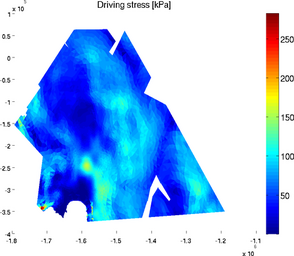
\includegraphics[width=\textwidth]{\assetsParentPath/assets/img/getting-started/plotting/matlab/driving_stress.png}
	\end{center}
\end{figure}
%}}}
\paragraph{elementnumbering}%{{{
In the debugging process, it is often very useful to display all the elements next to their numbers. This is what the special plot \lstinlinebg|'elementnumbering'| does:
\begin{lstlisting}
>> plotmodel(md, 'data', 'elementnumbering')
\end{lstlisting}
\begin{figure}[H]
	\begin{center}
		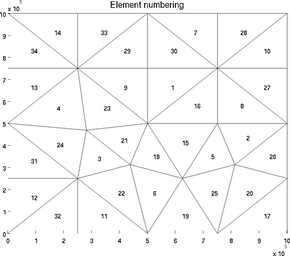
\includegraphics[width=\textwidth]{\assetsParentPath/assets/img/getting-started/plotting/matlab/elementnumbering.png}
	\end{center}
\end{figure}
A given list of elements can be highlighted with the \lstinlinebg|'highlight'| option:
\begin{lstlisting}
>> plotmodel(md, 'data', 'elementnumbering', 'highlight', [3 4 5 6 7])
\end{lstlisting}
\begin{figure}[H]
	\begin{center}
		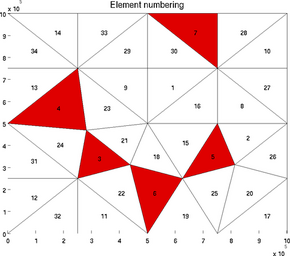
\includegraphics[width=\textwidth]{\assetsParentPath/assets/img/getting-started/plotting/matlab/elementnumbering_highlight.png}
	\end{center}
\end{figure}
%}}}
\paragraph{elements\_type}%{{{
The special plot \lstinlinebg|'elements_type'| displays the elements with a specific color for each formulation:
\begin{lstlisting}
>> plotmodel(md, 'data', 'elements_type')
\end{lstlisting}
\begin{figure}[H]
	\begin{center}
		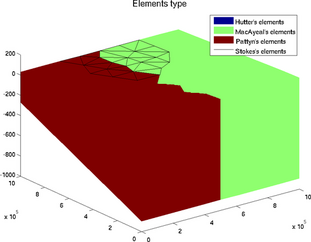
\includegraphics[width=\textwidth]{\assetsParentPath/assets/img/getting-started/plotting/matlab/elements_type.png}
	\end{center}
\end{figure}
%}}}
\paragraph{vertexnumbering}%{{{
In the debugging process, it is often very useful to display all the vertices next to their numbers. This is what the special plot \lstinlinebg|'vertexnumbering'| does:
\begin{lstlisting}
>> plotmodel(md, 'data', 'vertexnumbering')
\end{lstlisting}
\begin{figure}[H]
	\begin{center}
		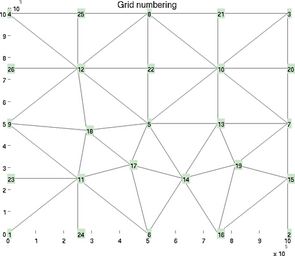
\includegraphics[width=\textwidth]{\assetsParentPath/assets/img/getting-started/plotting/matlab/gridnumbering.png}
	\end{center}
\end{figure}

A given list of vertices can be highlighted with the \lstinlinebg|'highlight'| option:
\begin{lstlisting}
>> plotmodel(md, 'data', 'vertexnumbering', 'highlight', [2 5 7 12])
\end{lstlisting}
\begin{figure}[H]
	\begin{center}
		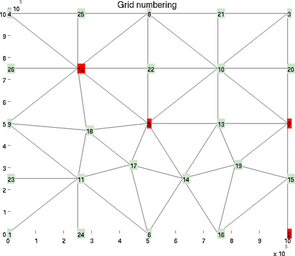
\includegraphics[width=\textwidth]{\assetsParentPath/assets/img/getting-started/plotting/matlab/gridnumbering_highlight.png}
	\end{center}
\end{figure}
%}}}
\paragraph{highlightelements}%{{{
The special plot \lstinlinebg|'highlightelements'| is very similar to the plot \lstinlinebg|'elementnumbering'|. It is another possibility to highlight one or several grids, but without indicating the number of all the elements. It is a lot faster for large models:
\begin{lstlisting}
>> plotmodel(md, 'data', 'highlightelements', 'highlight', 5)
\end{lstlisting}
\begin{lstlisting}
>> plotmodel(md, 'data', 'highlightelements', 'highlight', [5 12])
\end{lstlisting}
\begin{figure}[H]
	\begin{center}
		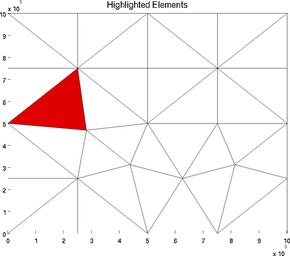
\includegraphics[width=0.475\textwidth]{\assetsParentPath/assets/img/getting-started/plotting/matlab/highlightelements_highlight.png}
		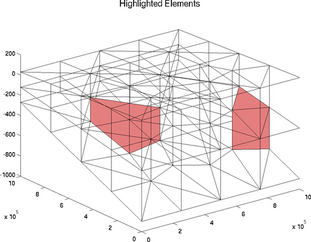
\includegraphics[width=0.475\textwidth]{\assetsParentPath/assets/img/getting-started/plotting/matlab/highlightelements_highlight3d.png}
	\end{center}
\end{figure}
%}}}
\paragraph{highlightgrids}%{{{
The special plot \lstinlinebg|'highlightgrids'| is very similar to \lstinlinebg|'gridnumbering'|. It is another possibility to highlight grids without indicating all the grids numbers. It is a lot faster for big models:
\begin{lstlisting}
>> plotmodel(md, 'data', 'highlightgrids', 'highlight', [12 20])
\end{lstlisting}
\begin{lstlisting}
>> plotmodel(md, 'data', 'highlightgrids', 'highlight', [12 16 26])
\end{lstlisting}
\begin{figure}[H]
	\begin{center}
		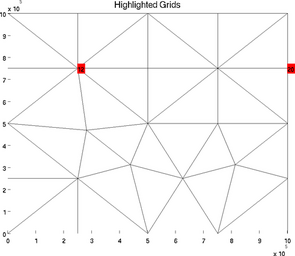
\includegraphics[width=0.475\textwidth]{\assetsParentPath/assets/img/getting-started/plotting/matlab/highlightgrids_highlight.png}
		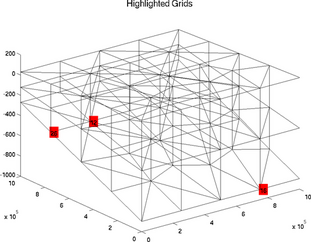
\includegraphics[width=0.475\textwidth]{\assetsParentPath/assets/img/getting-started/plotting/matlab/highlightgrids_highlight3d.png}
	\end{center}
\end{figure}
%}}}
\paragraph{icefront}%{{{
The special plot \lstinlinebg|'icefront'| displays the Neumann boundary conditions, i.e. all the segments on ice front and the normal to these segments, for a 2D or 3D mesh:
\begin{lstlisting}
>> plotmodel(md, 'data', 'icefront')
\end{lstlisting}
\begin{figure}[H]
	\begin{center}
		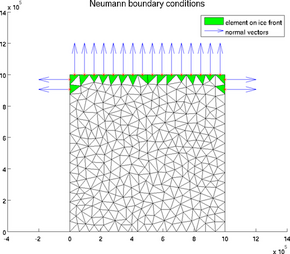
\includegraphics[width=0.475\textwidth]{\assetsParentPath/assets/img/getting-started/plotting/matlab/icefront2d.png}
		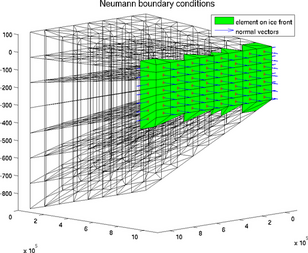
\includegraphics[width=0.475\textwidth]{\assetsParentPath/assets/img/getting-started/plotting/matlab/icefront3d.png}
	\end{center}
\end{figure}
%}}}
\paragraph{mesh}%{{{
The special plot \lstinlinebg|'mesh'| displays the mesh of 2D or 3D model:
\begin{lstlisting}
>> plotmodel(md, 'data', 'mesh')
\end{lstlisting}
\begin{figure}[H]
	\begin{center}
		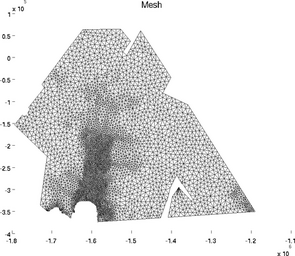
\includegraphics[width=0.475\textwidth]{\assetsParentPath/assets/img/getting-started/plotting/matlab/mesh2d.png}
		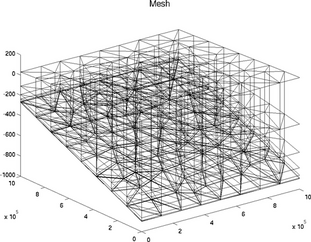
\includegraphics[width=0.475\textwidth]{\assetsParentPath/assets/img/getting-started/plotting/matlab/mesh3d.png}
	\end{center}
\end{figure}
%}}}
%}}}
\subsubsection{Quiver plot}%{{{
For 2D or 3D fields, a generic color plot cannot be used (except component by component). The \lstinlinebg|'data'| used by the function \lstinlinebg|plotmodel| must be a matrix of 2 or 3 columns. For example:
\begin{lstlisting}
>> plotmodel(md, 'data', [md.vx md.vy])
\end{lstlisting}
\begin{figure}[H]
	\begin{center}
		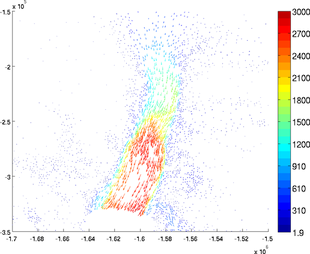
\includegraphics[width=\textwidth]{\assetsParentPath/assets/img/getting-started/plotting/matlab/plotquiver.png}
	\end{center}
\end{figure}

\paragraph{ColorLevels}
The number of colors can be chosen by using the \lstinlinebg|'colorlevels'| options. The user can specify a number of levels or a cell containing the values of color changes. For example:
\begin{lstlisting}
>> plotmodel(md, 'data', [md.vx md.vy], 'colorlevels', 3)
\end{lstlisting}
\begin{lstlisting}
>> plotmodel(md, 'data', [md.vx md.vy], 'colorlevels', 100)
\end{lstlisting}
\begin{figure}[H]
	\begin{center}
		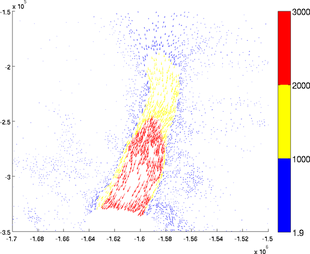
\includegraphics[width=0.475\textwidth]{\assetsParentPath/assets/img/getting-started/plotting/matlab/color3.png}
		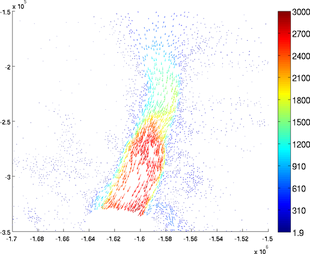
\includegraphics[width=0.475\textwidth]{\assetsParentPath/assets/img/getting-started/plotting/matlab/color100.png}
	\end{center}
\end{figure}
\begin{lstlisting}
>> plotmodel(md, 'data', [md.vx md.vy], 'colorlevels', {100, 200, 500, 1000, 2000, 2500})
\end{lstlisting}
\begin{figure}[H]
	\begin{center}
		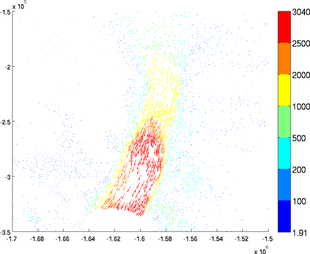
\includegraphics[width=\textwidth]{\assetsParentPath/assets/img/getting-started/plotting/matlab/colorcell.png}
	\end{center}
\end{figure}

\paragraph{Scaling}
The arrows length can be modified with the \lstinlinebg|'scaling'| options. The default value is 0.4. A higher scaling value will result in longer arrows:
\begin{lstlisting}
>> plotmodel(md, 'data', [md.vx md.vy], 'scaling', 1)
\end{lstlisting}
\begin{lstlisting}
>> plotmodel(md, 'data', [md.vx md.vy], 'scaling', 0.1)
\end{lstlisting}
\begin{figure}[H]
	\begin{center}
		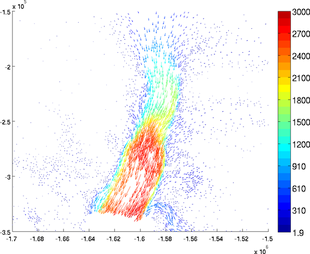
\includegraphics[width=0.475\textwidth]{\assetsParentPath/assets/img/getting-started/plotting/matlab/scaling1.png}
		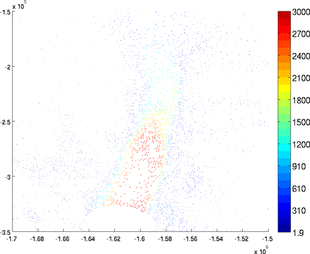
\includegraphics[width=0.475\textwidth]{\assetsParentPath/assets/img/getting-started/plotting/matlab/scaling01.png}
	\end{center}
\end{figure}

\paragraph{Autoscale}
If the user wants all the arrows to have the same length, use the option \lstinlinebg|'autoscale'| set as \lstinlinebg|'off'|:
\begin{lstlisting}
>> plotmodel(md, 'data', [md.vx md.vy], 'autoscale', 'off')
\end{lstlisting}
\begin{figure}[H]
	\begin{center}
		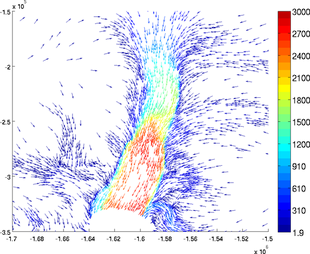
\includegraphics[width=\textwidth]{\assetsParentPath/assets/img/getting-started/plotting/matlab/autoscale.png}
	\end{center}
\end{figure}

\paragraph{Density}
The number of arrows can be reduced with the option \lstinlinebg|'density'|. If the density is set as 3, only one arrow out of 3 will be displayed. This option is very useful when the mesh is very refined:
\begin{lstlisting}
>> plotmodel(md, 'data', [md.vx md.vy], 'density', 3)
\end{lstlisting}
\begin{figure}[H]
	\begin{center}
		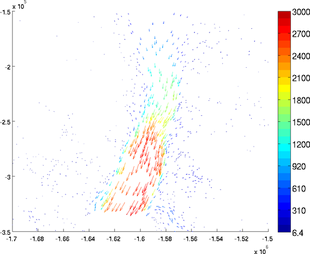
\includegraphics[width=\textwidth]{\assetsParentPath/assets/img/getting-started/plotting/matlab/density3.png}
	\end{center}
\end{figure}
%}}}
\subsubsection{Cross section}%{{{
The section plot can be used to display the value of a field on a given track. The option \lstinlinebg|'sectionvalue'| must be followed by the name of an ARGUS file which contained the coordinates of the points describing the profile (this file can be generated by \lstinlinebg|exptool.m|). The resulting plot will be a curve in 2D and a colored surface in 3D. For example:
\begin{lstlisting}
>> plotmodel(md, 'data', md.vel, 'expdisp', 'track.exp')
\end{lstlisting}
\begin{figure}[H]
	\begin{center}
		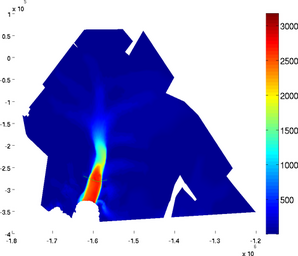
\includegraphics[width=\textwidth]{\assetsParentPath/assets/img/getting-started/plotting/matlab/track.png}
	\end{center}
\end{figure}
\begin{lstlisting}
>> plotmodel(md, 'data', md.vel, 'sectionvalue', 'track.exp')
\end{lstlisting}
\begin{figure}[H]
	\begin{center}
		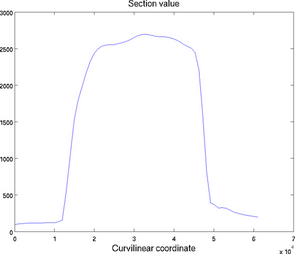
\includegraphics[width=0.475\textwidth]{\assetsParentPath/assets/img/getting-started/plotting/matlab/2d.png}
		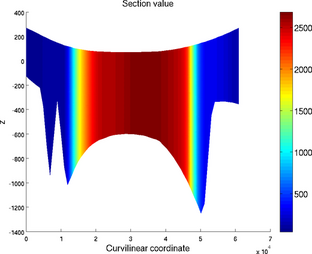
\includegraphics[width=0.475\textwidth]{\assetsParentPath/assets/img/getting-started/plotting/matlab/3d.png}
		\caption{Section plot for 2D (left) and 3D (right) models}
	\end{center}
\end{figure}

\paragraph{Resolution}
The horizontal and vertical (in 3D) resolution can be specified by the \lstinlinebg|'resolution'| option. It must be a list with the horizontal resolution followed by the vertical resolution (in meters). When not specified, the default resolution is displayed:
\begin{lstlisting}
>> plotmodel(md, 'data', md.vel, 'sectionvalue', 'track.exp', 'resolution', [2*10^4 0])
\end{lstlisting}
\begin{lstlisting}
>> plotmodel(md, 'data', md.vel, 'sectionvalue', 'track.exp', 'resolution', [10^3 0])
\end{lstlisting}

\paragraph{Show section}
The profile used to create the section plot can be also plotted with the \lstinlinebg|'showsection'| option:
\begin{lstlisting}
>> plotmodel(md, 'data', md.vel, 'showsection', 'on')
\end{lstlisting}
\begin{figure}[H]
	\begin{center}
		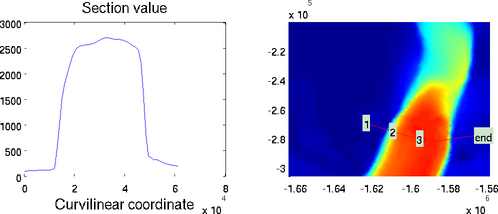
\includegraphics[width=\textwidth]{\assetsParentPath/assets/img/getting-started/plotting/matlab/show.png}
	\end{center}
\end{figure}
%}}}

\clearpage % Make sure all figures are placed before next section
